\documentclass{article}
\usepackage[utf8]{inputenc}
\usepackage{graphicx}
\addtolength{\oddsidemargin}{-.875in}
	\addtolength{\evensidemargin}{-.875in}
	\addtolength{\textwidth}{1.75in}

	\addtolength{\topmargin}{-.875in}
	\addtolength{\textheight}{1.75in}
\title{Sampling HW 5}
\author{Macenna Cowen }
\date{December 2018}

\begin{document}

\maketitle

\section{5.5}
A corporation wishes to obtain information on the effectiveness of a business machine. A number of division heads will be interviewed by telephone and asked to rate the equipment on a numerical scale. The divisions are located in North America, Europe, and Asia. Hence, stratified sampling is used. The costs are larger for interviewing division heads located outside of North America. The accompanying table gives the costs per interview, appropriate variances of the ratings, and the N that have been established. The corporation wants to estimate the average rating with $V(\bar{y_{st}}) = .1.$ Choose the sample size n that achieves this bound, and find the appropriate allocation. 
\begin{center}
    \begin{tabular}{|c|c|c|}
        \hline
        {Stratum I & Stratum II & Stratum III \\
        (North America) & (Europe) & (Asia)} \\
        \hline
       $c_1 = \$9 & c_2 = \$25 & c_3 = \$36 $\\
       $\sigma_1^2 = 2.25 & \sigma_2^2 = 3.24 & \sigma_3^2 = 3.24 $\\
       $N_1 = 112 & N_2 = 68 & N_3 = 39 $\\
        \hline 
        $SD = 1.5 & SD = 1.8 & SD = 1.8 $\\ 
        \hline
        $b_1 = 56 & b_2 = 24.48 & b_3 = 11.7 $\\
        \hline
    \end{tabular}
\end{center}
\begin{center}
    Allocation: Optimum \\
    $n_i \hspace{.25cm} \alpha \hspace{.25cm} \frac{N_i \sigma_i}{\sqrt{c_i}} = \hspace{.25cm} b_i \hspace{.25cm} \Rightarrow \hspace{.25cm} n_i \hspace{.2cm}\alpha \hspace{.2cm} b_i  $\\
    \smallskip
    $n_1 \alpha \frac{(112)(1.5)}{\sqrt{9}} \hspace{.2cm} = 56 = b_1 \hspace{1cm} n_2 \hspace{.2cm} \alpha \hspace{.2cm} \frac{(68)(1.8)}{\sqrt{25}} = 24.48 = b_2 \hspace{1cm} n_3 \hspace{.2cm} \alpha \hspace{.2cm} \frac{(39)(1.8)}{\sqrt{36}} = 11.7 = b_3 $\\
    \smallskip
    $\Rightarrow b_L = 92.18 $\\ 
    \smallskip
    $a_1 = \frac{56}{92.18} = .60751 \hspace{.7cm} a_2 = \frac{24.48}{92.18} = .26557 \hspace{.7cm} a_3 = \frac{11.7}{92.18} = .12693 \hspace{.7cm} \Rightarrow (n_i \alpha a_i) $ \\
    \smallskip
    $c = b_1 + b_2 + b_3 \Rightarrow c_L = 70 $\\
    \smallskip
    Replace $n_i$ by $kb_i$ and solve for k. \\
    \smallskip
    $k_1 b_1 c_1 + k_2 b_2 c_2 + k_3 b_3 c_3 = C_0 $\\
    \smallskip
    $k = \frac{C_0}{b_1 c_1 + b_2 c_2 + b_3 c_3} = \frac{70}{(504)(612)(421.2)} = .0000005388 $\\ 
    \smallskip
    $V(\bar{y_{st}} = .1 \Rightarrow B = 2\sqrt{.1} \Rightarrow B = .6325, B^2 = .4 $\\ 
    \smallskip
    $n' = \frac{(\sum N_K \sigma/\sqrt{c_K})(\sum N_i \sigma_i \sqrt{c_i})}{N^2 *D + \sum N_K \sigma_K^2} = \frac{(92.18)*(1537.2)}{47961(.1) + 598.68} = 26.27 \approx 26 $\\
    \smallskip
    $[n = 504+612+421.2 =1537.2 \hspace{1cm} D = \frac{B^2}{4} = .1] $\\
    \smallskip
    $\Rightarrow$ The allocated stratum size is $26$ when variance is bounded by $.1.$ 
    \smallskip
    $n_i = n (\frac{N_i \sigma_i/ \sqrt{c_i}}{\sum N_K \sigma_K / \sqrt{c_K}}) = \hspace{1cm} n_1 =  26(\frac{(112)(\sqrt{2.25})/\sqrt{9}}{92.18}) = 15.8 \approx 16 \hspace{1cm} n_2 = 6.9 \approx 7 \hspace{1cm} n_3 = 3.3 \approx 3 $\\
    \smallskip
    $\Rightarrow$ The allocated stratum sizes are: 16 for Stratum 1, 7 for Stratum 2, and 3 for Stratum 3. \\
\end{center}

\section{5.13}
A county government is interested in expanding the facilities of a day-care center for "mentally retarded children". The expansion will increase the cost of enrolling a child in the center. A sample survey will be conducted to estimate the proportion of families with "retarded" children that will make use of the expanded facilities. The families are divided into those who use the existing facilities and those who do not. Some families live in the city where the center is located, and some live in the surrounding suburban and rural areas. Thus, stratified random sampling is used, with users in the city, users in the surrounding area, nonusers in the city, and nonusers in the surrounding area, forming strata: $1$, $2$, $3$, and $4$, respectively. Approximately, 90\% of the present users and 50\% of the present nonusers will use the expanded facilities. The cost of obtaining an observation from a user is \$$4$ and from a nonuser is \$$8$. The difference in cost results is because nonusers are difficult to locate.\\
Existing records give: $N_1 = 97, N_2 = 43, N_3 = 145, N_4 = 68$. Find approximate sample size and allocation necessary to estimate the population proportion with a bound of $0.05$ on the error of estimation. \\
\begin{center}
    \begin{tabular}{|c|c|c|c|c|}
    \hline
     & S1 & S2 & S3 & S4 \\
      & Users+City & Users+Rural & Nonusers+City & Nonusers+Rural \\ 
     \hline
    c & \$4 & \$4 & \$8 & \$8 \\
    N & $N_1 = 97 & N_2 = 43 & N_3 = 145 & N_4 = 68$ \\
    p & $.9 & .9 & .5 & .5$ \\
    \hline
\end{tabular}
\end{center}
\begin{equation}
    a_i = (\frac{N_i \sqrt{\hat{p_i}\hat{q_i}/ c_i}}{\sum N_i \sqrt{\hat{p_i}\hat{q_i}/ c_i}})
\end{equation}
\begin{center}
    $a_1 = \frac{14.55}{58.653} = .248 \hspace{1cm} a_2 = \frac{6.45}{58.653} = .110 \hspace{1cm} a_3 = \frac{25.63}{58.653} = .437 \hspace{1cm} a_4 = \frac{12.02}{58.653} = .205 $ \\ 
\end{center}
\begin{center}
    $n = \frac{\sum N_i^2 p_i q_i / a_i}{N^2 D + \sum N_i p_i q_i} = \frac{22594.9159}{77.88+65.85} = 157.203 \approx 158 $
\end{center}
\begin{equation}
    n_i = na_i \\
\end{equation}
\begin{center}
    $n_1 = 38.9 \approx 39 \hspace{1cm} n_2 = 17.28 \approx 18 \hspace{1cm} n_3 = 68.7 \approx 69 \hspace{1cm} n_4 = 32.2 \approx 33 $ \\
\end{center}
Therefore, the sample size should consist of 158 families in order to get a bound of .05 on the error of estimation. And, the allotted stratum sample sizes should be 39 for S1, 17 for S2, 69 for S3, and 33 for S4. 

\section{5.15}
Suppose in exercise 5.13, that the total cost of sampling is fixed at $\$400$. Choose the sample size and allocation that minimizes the variance of the estimator $\hat{p_{st}}$ for this fixed cost. \\
\begin{equation}
    \frac{C_0}{c_1 a_1 + c_2 a_2 + c_3 a_3 + c_4 a_4} = K
\end{equation}
\begin{center}
    $K = \frac{400}{4(.248) + 4(.110) + 8(.437) + 8(.205)} = 60.903 $
\end{center}
\begin{equation}
    n_i = = ka_i \hspace{1 cm} n = \sum n_i \\ 
\end{equation}
\begin{center}
    $n_1 = (60.903)(.248) = 15.108 \approx 16 $ \\ 
    $n_2 = (60.903)(.110) = 6.697 \approx 7 $\\
    $n_3 = (60.903)(.437) = 26.616 \approx 27 $ \\
    $n_4 = (60.903)(.205) = 12.482 \approx 13 $ \\
    \smallskip
    $\hat{V}(\hat{p_{st}}) = (1- \frac{n}{N})(\frac{\hat{p}\hat{q}}{n-1}) \approx \hat{V}(\hat{p}) = (1- \frac{63}{353})(\frac{(.9)(.1)}{62}) = .069066437 $ \\ 
    $n_1 + n_2 + n_3 + n_4 = n \hspace{.5cm} \Rightarrow 16 + 7 + 27 + 13 = 63 = n  $
    \smallskip
    $B = 2\sqrt{\hat{V}(\hat{p})} = 2\sqrt{.001192543} = .069066437 $\\
\end{center}
With a fixed cost at \$400, the total sample size would be 63. The sample sizes would be: 16 for Stratum 1, 7 for Stratum 2, 27 for Stratum 3, and 13 for Stratum 4. With the error of estimation bounded by $.069066437$. \\ 

\section{2: 6.9}
A forest researcher is interested in estimating the number of dead fir trees in a 300-acre area of heavy infestation. Using an aerial photo, she divides the area into 200 1.5-acre plots. Let x denote the photo count of dead firs, and y the actual ground count for a simple random sample of n = 10 plots. The total number of dead fir trees obtained from the photo count is $ \tau_x = 4200$. Use the sample data in the accompanying table to estimate $\tau_y$, the total number of dead firs in the 300-acre area. Place a bound on the error of estimation. 
\smallskip
\begin{center}
    \begin{tabular}{|c|c|c|}
    \hline
    Plot Sampled & Photo Count & Ground Count \\
   $ n_i & x_i & y_i $\\
    \hline
    1 & 12 & 18 \\
    2 & 30 & 42 \\
    3 & 24 & 24 \\
    4 & 24 & 36 \\
    5 & 18 & 24 \\
    6 & 30 & 36 \\
    7 & 12 & 14 \\
    8 & 6 & 10 \\
    9 & 36 & 48 \\
    10 & 42 & 54 \\
    \hline
\end{tabular}
\end{center}
\begin{center}
    $r = \frac{\sum y_i}{\sum x_i} = \frac{306}{234} = 1.308 $ \\
    \smallskip
    $\Rightarrow$ Since the ratio is 1.308, that means the ground count estimated 30\% more dead trees than the photo showed. 
    \smallskip
    $\hat{\tau_y} = r(\tau_x) = (1.308)(4200) = 5493.6 \\$
    $\Rightarrow$ Estimated total number of dead trees for the ground count is 5494. \\
\end{center}
\begin{equation}
    \hat{V}(\hat{R_i}) = (1- \frac{n_i}{N_i})(\frac{s^2_ri}{\mu_x,i n_i}) \hspace{1cm} where, s_Ri^2 = \frac{\sum (y_{ij} - \hat{R_i}x{ij})^2} {n-1}
\end{equation}
\begin{center}
    $(1- \frac{10}{200}) \frac{12.0762654}{547.56(10)} = 45889.8 \hspace{1cm} s_{Ri}^2 = 12.0762654 $\\
    \smallskip
    $B = 2\sqrt{45889.8} = 428.43 \approx 429 = EB of \tau_y $\\
    \smallskip
    $\Rightarrow$ The total amount of trees is 45890, with a bound on the error of estimation being 429. So, between 45461 and 46319. 
\end{center}
Tapan's Additions: \\
\smallskip
I. Give a point estimate as well as a $95\%$ confidence interval for $R = \frac{\tau_y}{\tau_x}$ and interpret your results in the context of the problem. 
\begin{center}
    $R = \frac{\tau_y}{\tau_x} = \frac{5492.31}{4200} = 1.307 $\\
    \smallskip
    $CI = (.05, 1.307, 429) = .123744246 \Rightarrow (1.307 \pm .124) = (1.183, 1.431) \Rightarrow (18-43\% \text{Accurate}) $\\
    \smallskip
    $\Rightarrow$ $95\%$ confident that the ratio estimate $1.307$, between the intervals $1.183$ and $1.431$ is the actual ratio. 
\end{center}
II. Consider estimating $\mu_y$, the average number of dead fir trees per 1.5 acre plot, using 4 different methods: the sample mean (ch4), ratio estimation, regression estimation, and difference estimation. \\
Draw a scatter plot of the data along with a fixed straight line. What does that plot suggest about the suitability of the four methods estimating $\mu_y$? \\
\smallskip
\begin{figure}[h]
    \centering
    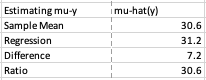
\includegraphics[width=6cm]{2iitable.png}
\end{figure}
\begin{figure}[h]
    \centering
    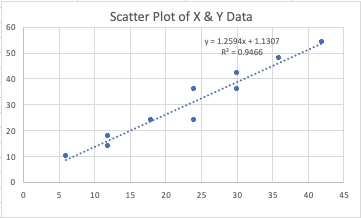
\includegraphics[width=6cm]{2iichart.png}
\end{figure}
\begin{center}
    $\Rightarrow$ The plot suggests that the ratio estimator should be used because the regression line looks like it's going to pass through 0. \\
\end{center}
III. Estimate $\mu_y$ using the four estimation methods from the last part of this question (II). For each estimator, calculate the error bound for each estimate. Put in a table. \\
\smallskip
\begin{center}
\begin{tabular}{|c|c|c|c|c|c|}
    \hline
    Estimator & $\hat{\mu_y}$ & $V(\hat{\mu_y})$ & $s^2$ & B & EB \\
    \hline
    Sample Mean & 30.6 & 1 & 0 & 2 & (28.6, 32.6) \\
    Regression & 31.2 & -1 & 400 & 2 & (29.2, 33.2) \\
    Difference & 7.2 & .7408 & 72 & 1.7214 & (5.49, 8.92) \\
    Ratio & 30.6 & 1 & 4.5438 & 2 & (28.6, 32.6) \\
    \hline
\end{tabular}
\end{center}

IV. Based on the numerical results in part (III), which of the following four methods would you suggest to use and why? \\ 
\begin{center}
    Based on the four estimation methods used to calculate $\mu_y$, I would suggest using the ratio estimation method because firstly, the variance of the ratio method is 1, secondly, the regression line on the scatter plot goes through 0, and thirdly, this estimator has the same sample mean value as the one from the sample mean estimation method, which is the most simplified estimation method. \\
\end{center}

V. Estimate $\tau_y$, the total number of dead fit trees, using the above four estimates and their error bounds in a table. \\
\smallskip
\begin{center}
\begin{tabular}{|c|c|c|c|c|c|c|}
    \hline
    Estimator & $\mu$ & $V(\mu)$ & $\tau_y$ & $V(\tau_y)$ & B & EB \\
    \hline
    Sample Mean & 30.6 & 0 & 6120 & 1349392 & 2323.267 & (3796.733, 8443.267) \\
    Regression & 31.2 & 3.103 & 5492.3077 & 17044.6355 & 261.1102 & (5231.197, 5753.418) \\
    Difference & 7.2 & 1.9591 & 1440 & 2821.12 & 106.2284 & (1333.772, 1546.228) \\
    Ratio & 30.6 & 1.1473 & 5492.3078 & 6301.0238 &158.758 & (5333.55, 5651.066) \\
    \hline
\end{tabular}
\smallskip
\end{center}

VI. If the ratio estimator is used, what should be the sample size for estimating $\mu_y$ with an error bound 1.5? \\
\smallskip
\begin{equation}
    n = \frac{N \sigma^2}{N D + \sigma^2} \hspace{1cm} D = \frac{B^2}{4}
\end{equation}
\begin{center}
    $n = \frac{(200)(12.076)}{(200)(.5625) + 12.076} = 19.39 \approx 20  \hspace{2cm} D = \frac{1.5^2}{4} $\\
    \smallskip
    $\Rightarrow$ The sample size should be 20 with an error bound of 1.5 if ratio estimation is used. \\
\end{center}
\smallskip
VII. Determine the necessary sample size for estimating the total number of dead trees $(\tau_y)$ using regression estimator and with error bound 300. \\

\begin{equation}
    n = \frac{(N)*(V(\tau_y))}{N *D + V(\tau_y)} \hspace{1cm} Where, \hspace{.5cm} D = \frac{B^2}{4 N^2} \\
\end{equation}
\begin{center}
    $n = \frac{200*13.24012}{200*.5625 + 13.24012} = 21.06 \approx 21 $ \hspace{2cm} $\hspace{1cm} D = \frac{300^2}{4} = .5625 $ \\
    \smallskip
    $\Rightarrow$ Through regression estimation, the sample size necessary to estimate the total number of dead fir trees is 21. \\
\end{center}
\end{document}

